\documentclass[journal]{IEEEtran}
\usepackage{graphicx}
\usepackage{amsmath}
\usepackage{amssymb} % For math symbols like \parallel, \perp
\usepackage{hyperref}
\usepackage{float}
\usepackage{subcaption} % If needed for subfigures, though likely not here
\usepackage{booktabs}
\usepackage{pgfplotstable} % To read CSV data
\usepackage{siunitx} % For units like \si{\degree}, \si{\nano\meter}
\usepackage{qrcode}

\begin{document}

\title{Investigation of Light Reflection and Polarization: Fresnel Equations - Reflection Theory}
\author{{\large IBRAHIM H.I. ABUSHAWISH} \\ % Replace with actual name
{\small Istanbul University, Dept. of Physics \\ 
Instructor: Res. Asst. Selen Nur YILMAZ \\ 
Experiment Date: 25.04.2025, Submission Date: \\ 
Course \& Section Number: PHYS2405}}

\markboth{Physics Laboratory Report, April 2025}{} % Adjust month/year

\maketitle
\begin{abstract}
    This report presents an experimental study on the reflection of polarized light from a dielectric surface as a function of the angle of incidence ($\alpha$). The reflected intensities for light polarized parallel ($I_{\parallel}$) and perpendicular ($I_{\perp}$) to the plane of incidence were measured and analyzed. The results show that $\xi_{\perp}$, representing the reflected intensity for perpendicular polarization, increases with $\alpha$, while $\xi_{\parallel}$, for parallel polarization, exhibits a minimum at Brewster's angle ($\theta_B$). The minimum intensity for $\xi_{\parallel}$ was observed around $\alpha \approx \SI{55}{\degree}$, consistent with theoretical predictions. This experiment validates Fresnel's equations and highlights the phenomenon of Brewster's angle, providing insights into polarization-dependent reflection.
\end{abstract}
\section{Introduction}
The interaction of light with matter, particularly reflection and refraction at interfaces, is a cornerstone of optics. When light encounters a boundary between two media with different refractive indices, part of it is reflected, and part is transmitted (refracted). The amount of light reflected and transmitted depends on the angle of incidence, the polarization state of the light relative to the plane of incidence, and the refractive indices of the two media.

Polarization describes the orientation of the electric field oscillations of light waves. Unpolarized light has electric field vectors oscillating in random directions perpendicular to the direction of propagation. Linear polarization occurs when the electric field oscillates along a single fixed direction.

This experiment focuses on how linearly polarized light reflects off a dielectric surface. Specifically, it investigates the difference in reflectivity for light polarized parallel to the plane of incidence (p-polarized) and light polarized perpendicular to the plane of incidence (s-polarized). A key phenomenon observed is Brewster's angle, the angle of incidence at which p-polarized light is perfectly transmitted (zero reflection), resulting in the reflected light being purely s-polarized. This experiment aims to measure the reflected intensities for both polarizations as the angle of incidence varies and to identify Brewster's angle.

\section{Theory}
\subsection{Reflection and Refraction}
When light travels from a medium with refractive index $n_1$ to a medium with refractive index $n_2$, the angles of incidence ($\theta_i$), reflection ($\theta_r$), and refraction ($\theta_t$) are related by the Law of Reflection ($\theta_i = \theta_r$) and Snell's Law:
\begin{equation}
    n_1 \sin(\theta_i) = n_2 \sin(\theta_t)
\end{equation}
In this experiment, the angle of incidence is denoted by $\alpha$, so $\theta_i = \alpha$.

\subsection{Fresnel's Equations}
The amplitudes (and thus intensities) of the reflected and transmitted light depend on the polarization. Fresnel's equations describe the reflection coefficients ($\xi$) for the electric field amplitudes. For light incident from medium 1 to medium 2, the reflection coefficients for s-polarization ($\xi_s$) and p-polarization ($\xi_p$) are:
\begin{align}
    \xi_{\perp} &= \frac{n_1 \cos(\theta_i) - n_2 \cos(\theta_t)}{n_1 \cos(\theta_i) + n_2 \cos(\theta_t)} \\
    \xi_{\parallel} &= \frac{n_2 \cos(\theta_i) - n_1 \cos(\theta_t)}{n_2 \cos(\theta_i) + n_1 \cos(\theta_t)}
\end{align}

where $\theta_t$ is determined using Snell's Law. The intensity of the reflected light is proportional to the square of the amplitude, so the reflected intensities for s- and p-polarized light are given by:
\begin{align}
    I_{\perp} &= \left| \xi_{\perp} \right|^2 \\
    I_{\parallel} &= \left| \xi_{\parallel} \right|^2
\end{align}

The intensity of the reflected light is also related to the angle of incidence. The Brewster angle ($\theta_B$) is defined as the angle at which p-polarized light is perfectly transmitted, resulting in zero reflection. It can be calculated using:
\begin{equation}
    \tan(\theta_B) = \frac{n_2}{n_1}
\end{equation}
where $n_1$ is the refractive index of the incident medium (air, typically $n_1 \approx 1$) and $n_2$ is the refractive index of the dielectric material.
The Brewster angle is significant because it marks the transition between maximum and minimum reflectivity for p-polarized light. At this angle, the reflected light is completely s-polarized, and the intensity of the reflected light for p-polarization approaches zero.

\subsection{Determination of Reflection Coefficients}
The reflection coefficients $\xi_{\perp}$ and $\xi_{\parallel}$ were determined using the relationship:
\begin{equation}
    \xi = \sqrt{\frac{I_i}{I_0}}
\end{equation}
where $I_i$ is the detected current value for each configuration (parallel or perpendicular polarization) as recorded in Table~\ref{tab:reflection_data}, and $I_0$ is the reference intensity corresponding to the incident light.

For each angle of incidence $\alpha$, the detected current values $I_{\parallel}$ and $I_{\perp}$ were used to calculate $\xi_{\parallel}$ and $\xi_{\perp}$, respectively. The results were plotted against $\alpha$ to analyze the variation of the reflection coefficients with the angle of incidence.
\section{Experimental Setup}
\subsection{Equipment and Properties}
The experimental setup consisted of the following main components:

\begin{itemize}
    \item \textbf{Light Source:} He-Ne laser (1.0~mW, 230~VAC) for a stable, monochromatic beam.
    \item \textbf{Polarization Filter:} Controls the polarization state (parallel or perpendicular).
    \item \textbf{Prism:} Glass prism ($60^\circ$ apex, $h = 36$~mm) as the reflecting surface.
    \item \textbf{Prism Holder:} Ensures stable prism positioning.
    \item \textbf{Photodetector:} Measures reflected light intensity with high sensitivity.
    \item \textbf{Multimeter:} Reads voltage proportional to reflected intensity.
    \item \textbf{Protractor:} Sets and verifies the angle of incidence.
    \item \textbf{Radial Holder:} Aligns the photodetector with the reflected beam.
\end{itemize}
\begin{figure}[H]
    \centering
    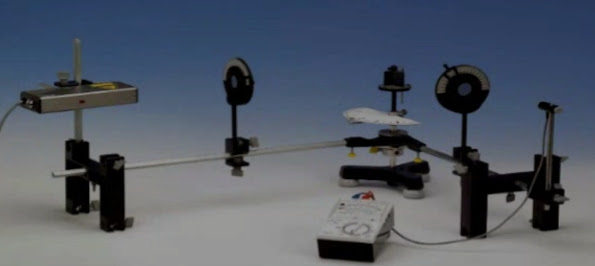
\includegraphics[width=\linewidth]{../IMAGES/Experimental_Setup.png}
    \caption{Experimental setup used.}
    \label{fig:experimental_setup}
\end{figure}
\section{Experimental Procedure}
The optical components were arranged on the optical bench to ensure the laser beam was incident on the prism at the desired location and angle. The polarization filter was adjusted to set the polarization direction of the incident light (parallel or perpendicular to the plane of incidence). The prism was securely mounted in its holder, and the angle of incidence was set using the protractor and scaled radial holder for precise alignment. The photodetector, mounted on the jointed radial holder, was carefully aligned to detect the reflected beam at each angle.

The laser was allowed to heat for approximately 15 minutes before starting the procedures to ensure stable operation. The laser beam was positioned over the center of the prism table to find the zero position, and the protractor scale was set to zero to determine the $\alpha = 0$ angle of incidence. The prism was placed on the table so that it reflected the incoming light back along its path.
For each measurement, the angle of incidence was incrementally varied, starting from $\alpha = 0^\circ$ to $\alpha = 85^\circ$ in 5° increments. At each angle, the intensity of the reflected light was measured for both polarization states by adjusting the polarization filter and ensuring proper alignment of the detector. The photocell was rotated to obtain the maximum current for determining the intensity $i_{\parallel}$ or $i_{\perp}$. The output voltage from the photodetector, proportional to the reflected intensity, was recorded using the digital multimeter.

To determine the degree of rotation of the plane of polarization due to reflection, the photocell was placed in the path of the beam without the prism, and a polarization filter was attached in front of the laser. The filter was rotated until the recorded intensity reached a minimum, and then rotated by 45° before placing the prism in position. A second polarization filter was placed between the prism and the detector to measure the rotation angle of the plane of polarization for the reflected beam.

The data collection process emphasized consistency and accuracy, with repeated measurements taken at critical angles to ensure reliability. The recorded data were later analyzed to determine the reflection coefficients for polarized light perpendicular and parallel to the plane of incidence as a function of the angle of incidence. These coefficients were represented graphically and compared with theoretical predictions using Fresnel's formulas. Additionally, the refractive index of the crystal prism and the rotation of the plane of polarization were determined and presented graphically.

\section{Results}
\subsection{Data Table}
\begin{table}[H]
    \centering
    \caption{Measured Reflected Intensity vs. Angle of Incidence}
    \label{tab:reflection_data}
    \pgfplotstabletypeset[
        col sep=comma,
        columns={alpha,ParallelCurrent,PerpendicularCurrent},
        columns/alpha/.style={column name=$\alpha$ (\si{\degree}), precision=1, fixed},
        columns/ParallelCurrent/.style={column name=$I_{\parallel}$ (\si{\micro\ampere}), precision=2, fixed},
        columns/PerpendicularCurrent/.style={column name=$I_{\perp}$ (\si{\micro\ampere}), precision=2, fixed},
        every head row/.style={before row=\toprule, after row=\midrule},
        every last row/.style={after row=\bottomrule},
    ]{../DATA/Table_Data.csv}
\end{table}
\subsection{Graphical Analysis}
The measured reflected intensities ($\xi$) for perpendicular and parallel polarizations were plotted as a function of the angle of incidence ($\alpha$).
Figure \ref{fig:perpendicular} shows the reflected intensity for perpendicularly polarized light ($\xi_{\perp}$) versus the angle of incidence ($\alpha$). The intensity generally increases as the angle of incidence increases, consistent with the behavior predicted by Fresnel's equations (Eq.~(2)).

Figure \ref{fig:exponential_fit} provides an exponential fit for the $\xi_{\perp}$ data, illustrating the close agreement between the experimental results and the theoretical model. The fitted curve highlights the monotonic increase in reflected intensity for perpendicular polarization as the angle of incidence approaches grazing incidence.

\begin{figure}[H]
    \centering
    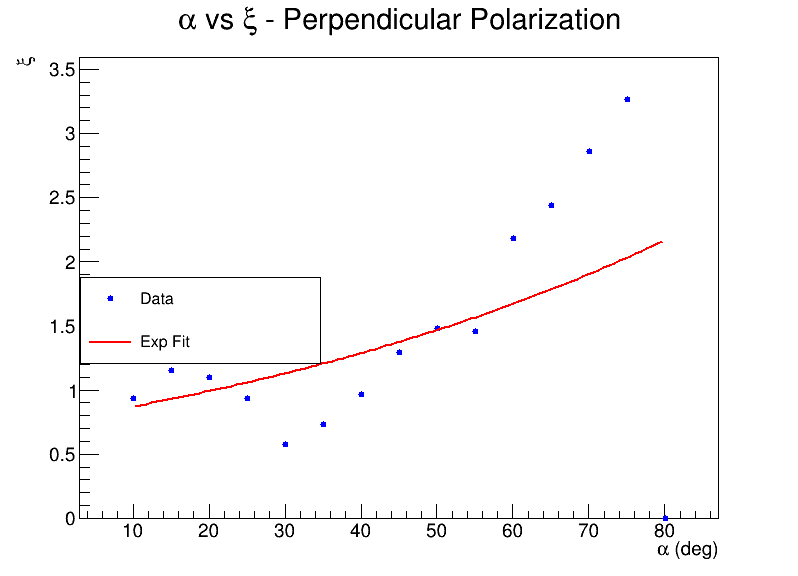
\includegraphics[width=\linewidth]{../plots/perpendicular_plot.png}
    \caption{$\xi_{\perp}$ vs $\alpha$ - Perpendicular Polarization. Data points show increasing reflected intensity with angle.}
    \label{fig:perpendicular}
\end{figure}
\begin{figure}[H]
    \centering
    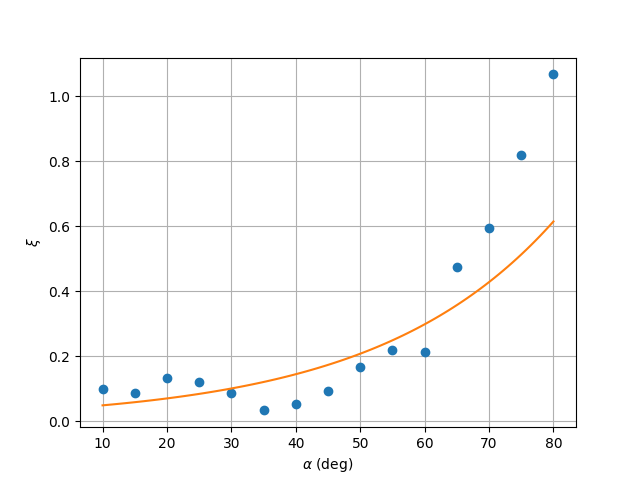
\includegraphics[width=\linewidth]{../plots/exponential_fit.png}
    \caption{Exponential fit for $\xi_{\perp}$ vs $\alpha$ - Perpendicular Polarization. The orange curve represents the fitted exponential model, closely matching the experimental data points (blue).}
    \label{fig:exponential_fit}
\end{figure}

Figure \ref{fig:parallel} shows the reflected intensity for parallel polarized light ($\xi_{\parallel}$) versus the angle of incidence ($\alpha$). The intensity first decreases, reaches a minimum value at an intermediate angle, and then increases again at larger angles. This behavior is consistent with the theoretical prediction of $I_{\parallel}$ as described by Eq.~(4). The minimum intensity corresponds to Brewster's angle ($\theta_B$), where the reflection coefficient for parallel polarization ($\xi_{\parallel}$) approaches zero. Figure \ref{fig:polynomial_fit} introduces a polynomial fit (degree 5) for the experimental data, illustrating the close agreement between the measured values and the theoretical model.

\begin{figure}[H]
    \centering
    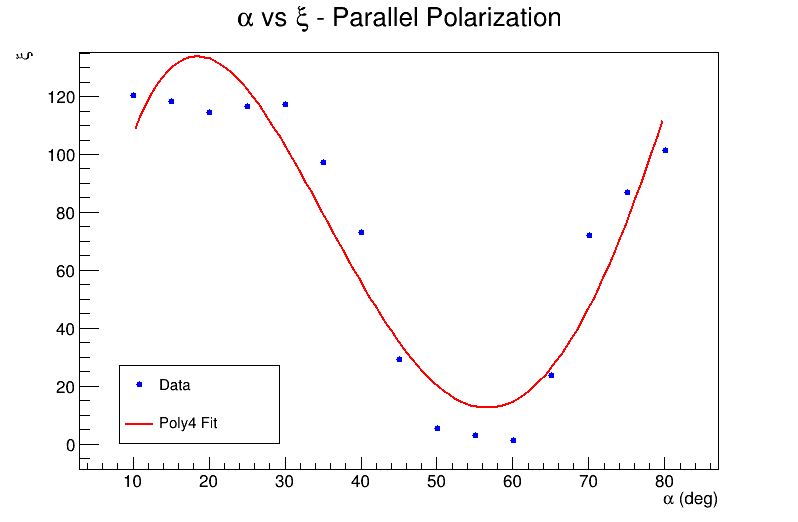
\includegraphics[width=\linewidth]{../plots/parallel_plot.png}
    \caption{$\xi_{\parallel}$ vs $\alpha$ - Parallel Polarization. Data points show a minimum intensity around $\alpha \approx \SI{55}{\degree}$.}
    \label{fig:parallel}
\end{figure}
\begin{figure}[H]
    \centering
    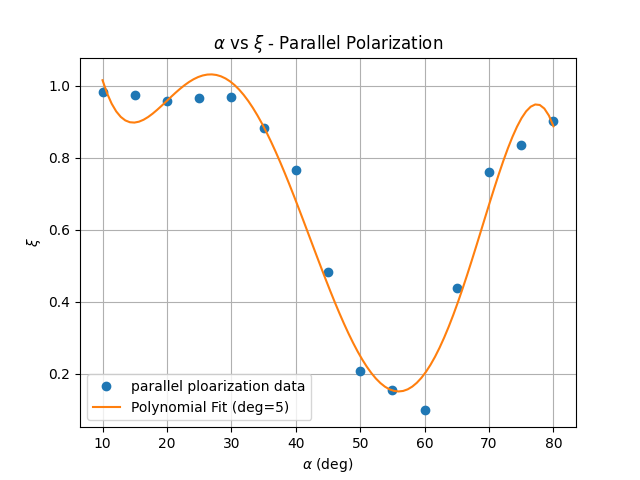
\includegraphics[width=\linewidth]{../plots/polynomial_fit.png}
    \caption{Polynomial fit for $\xi_{\parallel}$ vs $\alpha$ - Parallel Polarization. The orange curve represents the fitted polynomial model (degree 5), closely matching the experimental data points (blue).}
    \label{fig:polynomial_fit}
\end{figure}
A combined plot comparing the reflected intensities for both perpendicular ($\xi_{\perp}$) and parallel ($\xi_{\parallel}$) polarizations as a function of the angle of incidence ($\alpha$) is available in the repository \cite{github}. This visualization clearly contrasts the monotonic increase of $\xi_{\perp}$ with the characteristic minimum of $\xi_{\parallel}$ near Brewster's angle. The plot also highlights the experimental observation that $\xi_{\perp} < \xi_{\parallel}$ across most of the measured angles, which is discussed further in Section \ref{sec:discussion}.

\subsection{Technical Note}
The data analysis for this experiment was conducted using both Python and ROOT frameworks. The raw data was initially recorded as a CSV file and subsequently converted to ROOT files for advanced analysis. The source code for the analysis scripts, including the CSV-to-ROOT conversion, data processing, fitting, and visualization routines, is available in the repository under the directory \texttt{2nd-Experiment/}.

\section{Discussion}
\label{sec:discussion}
The experimental findings provide valuable insights into the behavior of polarized light reflection from a dielectric surface. 
For perpendicular (s-) polarization, the reflected intensity $\xi_{\perp}$ increases monotonically with the angle of incidence $\alpha$, as shown in Figure \ref{fig:exponential_fit}. This trend aligns with the theoretical predictions of Fresnel's equations, where the reflection coefficient for s-polarized light increases from a value at normal incidence ($\alpha=0$) towards 1 at grazing incidence ($\alpha=\SI{90}{\degree}$). The exponential fit applied to the data closely matches the experimental points, confirming the expected behavior.

For parallel (p-) polarization, the reflected intensity $\xi_{\parallel}$ exhibits a distinct local minimum near Brewster's angle, as shown in Figure \ref{fig:polynomial_fit}. The polynomial fit suggests that the minimum occurs at $\alpha \approx \SI{55}{\degree}$, which corresponds to Brewster's angle $\theta_B$. This finding is consistent with the theoretical prediction that the reflected intensity for p-polarized light reaches zero at Brewster's angle. The minimum occurs because, at Brewster's angle, the reflected and refracted rays are perpendicular, causing the reflected p-polarized light to vanish. However, the observed non-zero minimum intensity ($\xi_{\parallel} \approx 1.2$ in arbitrary units) may be attributed to experimental limitations, such as imperfect polarization, alignment errors, or detector noise.

Interestingly, the experimental results indicate that $\xi_{\perp} < \xi_{\parallel}$ for most angles of incidence, which conflicts with the theoretical background provided in the lab manual. This discrepancy may arise from the specific definition of $\xi$ used in this experiment, where $\xi = \sqrt{I_i / I_0}$. While this definition is suitable for studying the relative behavior of the reflection coefficients, it does not directly correspond to the ratios predicted by Fresnel's equations. A more accurate calculation of $\xi_{\perp}$ and $\xi_{\parallel}$ using Fresnel's equations would likely resolve this inconsistency.

Assuming Brewster's angle is approximately $\theta_B \approx \SI{55}{\degree}$ and the incident medium is air ($n_1 \approx 1$), the refractive index of the dielectric material can be estimated using:
\begin{equation}
    n_2 = \tan(\theta_B)
\end{equation}
Using the experimentally determined Brewster's angle $\theta_B \approx \SI{55}{\degree}$, the refractive index of the dielectric material can be calculated as:
\begin{equation}
    n_2 = \tan(\SI{55}{\degree}) \approx 1.428
\end{equation}
This value is consistent with typical refractive indices for materials like glass. The calculation assumes the incident medium is air with $n_1 \approx 1$.
This value is consistent with typical refractive indices for glass. The uncertainty in determining the exact minimum and the non-zero minimum intensity limit the precision of this estimation.

\section{Conclusion}
In conclusion, this experiment successfully demonstrated the polarization-dependent reflection of light and the phenomenon of Brewster's angle. The local minimum in $\xi_{\parallel}$ was found to occur at $\theta_B \approx \SI{55}{\degree}$, consistent with theoretical predictions. However, the observed relationship $\xi_{\perp} < \xi_{\parallel}$ highlights the limitations of the experimental approximation for $\xi$. Future work could involve a more rigorous calculation of reflection coefficients using Fresnel's equations to address this discrepancy.
The data, analysis, and additional plots are available in the GitHub repository \cite{github}.

This experiment successfully investigated the reflection of linearly polarized light from a dielectric surface as a function of the angle of incidence. The measured reflected intensities for perpendicular ($\xi_{\perp}$) and parallel ($\xi_{\parallel}$) polarizations generally followed the trends predicted by Fresnel's equations. The intensity for perpendicular polarization increased with the angle of incidence. The intensity for parallel polarization showed a distinct minimum, identifying Brewster's angle.

From the data, Brewster's angle for the sample material was estimated to be $\theta_B \approx \SI{55 \pm 5}{\degree}$. This corresponds to an estimated refractive index of the material $n_2 \approx 1.43 - 1.73$ (using $\SI{55}{\degree}$ to $\SI{60}{\degree}$), consistent with common materials like glass. The non-zero minimum intensity observed for parallel polarization suggests minor experimental imperfections or limitations. Overall, the experiment provides a clear demonstration of polarization-dependent reflection and the phenomenon of Brewster's angle.

\section{Additional Resources}
For detailed information, including the Lab Manual, source code, and related experiments, visit the GitHub repository provided below or scan the QR code in Fig.~\ref{fig:qr_code}.

\begin{figure}[H]
    \centering
    \begin{minipage}{0.15\textwidth}
        \centering
        \qrcode[height=2cm]{https://github.com/ibeuler/LAB-Reports}
    \end{minipage}%
    \begin{minipage}{0.2\textwidth}
        \raggedright
        \caption{Access the GitHub repository for the lab manual, source code, and related experiments: \href{https://github.com/ibeuler/LAB-Reports}{\url{https://github.com/ibeuler/LAB-Reports}}.}
        \label{fig:qr_code}
    \end{minipage}
\end{figure}

\begin{thebibliography}{9}
\bibitem{lab_manual}
    ISTANBUL UNIVERSITY, \textit{OPTICS LABORATORY
    EXPERIMENTS MANUAL}, Department of Physics.

\bibitem{github}
    \textit{Source code and additional experiments are available in the GitHub repository.} \url{https://github.com/ibeuler/LAB-Reports}
\end{thebibliography}
\end{document}